\documentclass[12pt]{article}
\usepackage{mathtools,amsthm,amssymb,icomma,upgreek,xfrac}
\mathtoolsset{showonlyrefs,mathic}

\usepackage[utf8]{inputenc}
\usepackage{polski}
\usepackage[condensed,math]{}
\usepackage[T1]{fontenc}
\usepackage[hidelinks,breaklinks,pdfusetitle,pdfdisplaydoctitle]{hyperref}
\usepackage{tikz}
\usepackage{graphicx}
\usepackage{multirow}
\usepackage{longtable}
\usepackage{minted}


\begin{document}
	\begin{center}
		\begin{LARGE}
			\textbf{Projekt 1}
		\end{LARGE}
	\end{center}
	\begin{center}
		\begin{Large}
			\textbf{Modulacje i synteza wybranych sygnałów}
		\end{Large}
	\end{center}
	\newpage
	\section{Generowanie sygnałów}
	W tym projekcie wykonamy modulacje amplitudy, fazy i częstotliwości oraz syntezę sygnału prostokątnego, trójkątnego i piłokształtnego. Zacznijmy od napisania funkcji w Scilabie. W tym celu wykorzystamy następujące wzory na sygnały o okresie $T$ i amplitudzie $A$:
	\begin{itemize}
		\item sygnał prostokątny
		\[
			x(t) = A\cdot \text{sgn}\left(\sin\frac{2\pi t}{T}\right),
		\]
		\item sygnał trójkątny
		\[
			x(t) = 2A\left|\frac{t}{T} - \left\lfloor \frac{t}{T} + \frac{1}{2} \right\rfloor \right| - A,
		\]
		\item sygnał piłokształtny
		\[
			x(t) = 2A\left(\frac{t}{T} - \left\lfloor \frac{t}{T} + \frac{1}{2} \right\rfloor \right).
		\]
	\end{itemize}
	Teraz przepiszemy te funkcje do Scilaba:
	
	Sygnał prostokątny:
	\begin{minted}[linenos, fontsize=\small]{scilab}
		function x = rectangular(A, t, T)
		x = A * sign(sin(2 * %pi * (t/T)));
		endfunction
	\end{minted}
	Sygnał trójkątny:
	\begin{minted}[linenos, fontsize=\small]{scilab}
		function x = triangular(A, t, T)
		x = 2*A*(abs(2*(t/T - floor(t/T + 0.5)))) - A;
		endfunction
	\end{minted}
	Sygnał piłokształtny:
	\begin{minted}[linenos, fontsize=\small]{scilab}
		function x = sawtooth(A, t, T)
		x = 2*A*(t/T - floor(t/T + 0.5));
		endfunction
	\end{minted}
	\section{Synteza sygnału}
	Do wykonania syntez sygnałów posłużymy się współczynnikami rozwinięcia szeregu geometrycznego Fouriera
	\[
		f(t) = \frac{a_0}{2} + \sum_{n=1}^{\infty}\left[a_n\cos\left(\frac{2\pi n t}{T}\right)+b_n\sin\left(\frac{2\pi nt}{T}\right)\right],
	\]
	gdzie
	\[
		a_n =\frac{2}{T} \int_{-T/2}^{T/2}f(t)\cos\left(\frac{2\pi nt}{T}\right)dt,
	\]
	\[
		b_n = \frac{2}{T} \int_{-T/2}^{T/2}f(t)\sin\left(\frac{2\pi nt}{T}\right)dt.
	\]
	Algorytm wyliczania współczynników opiera się na obliczaniu ich w odstępach o określonym kroku czasowym, stąd ze względu na dyskretny charakter tej funkcji zamiast całki posłużymy się sumą. Poniżej zamieszczony został algorytm napisany w Scilabie.
	\begin{minted}[linenos, fontsize=\small]{scilab}
		function synthesis(NF, NT, x)
		//NF - liczba składników harmonicznych do przybliżania sygnału
		//NT - liczba okresów
		//x - wykorzystana funkcja fali
		
		T = 1;                  //okres
		N_per = 1000;           //liczba próbek na 1 okres
		N = N_per * NT;         // całkowita liczba próbek
		dt = (T * NT) / N;      //krok czasowy
		A = 1;                  //amplituda
		t = 0:dt:(T*NT - dt);   //oś czasu
		
		//generowanie funkcji fali z zadanymi parametrami
		xn = x(A, t, T)
		
		//obliczanie współczynników szeregu Fouriera
		a0 = sum(xn)*dt/(T*NT);
		an = zeros(1, NF);
		bn = zeros(1, NF);  
		
		for n = 1:NF
		an(n) = 2*sum(xn.*cos(2*%pi*n*t/T))*dt/(T*NT);
		bn(n) = 2*sum(xn.*sin(2*%pi*n*t/T))*dt/(T*NT);
		end
		
		//tworzenie sygnału za pomocą szeregu Fouriera
		y = zeros(1, N);
		for n = 1:NF
		y = y + an(n)*cos(2*%pi*n*t/T) +  bn(n)*sin(2*%pi*n*t/T);
		end
		
		//rysowanie wykresu funkcji fali
		plot(t,xn);
		//rysowanie sygnału wygenerowanego za pomocą szeregu Fouriera   
		plot(t,y,'r');      
		xlabel('czas (sek)');
		ylabel('Amplituda');
		endfunction
	\end{minted}
	Poniżej znajdują się wykresy wygenerowane przez wywołanie następujących funkcji.
	\newpage
	Sygnał prostokątny
	\begin{minted}[linenos, fontsize=\small]{scilab}
		synthesis(50, 3, rectangular)
	\end{minted}
	\begin{figure}[H]
		\centering
		\hspace*{-4.5cm}
		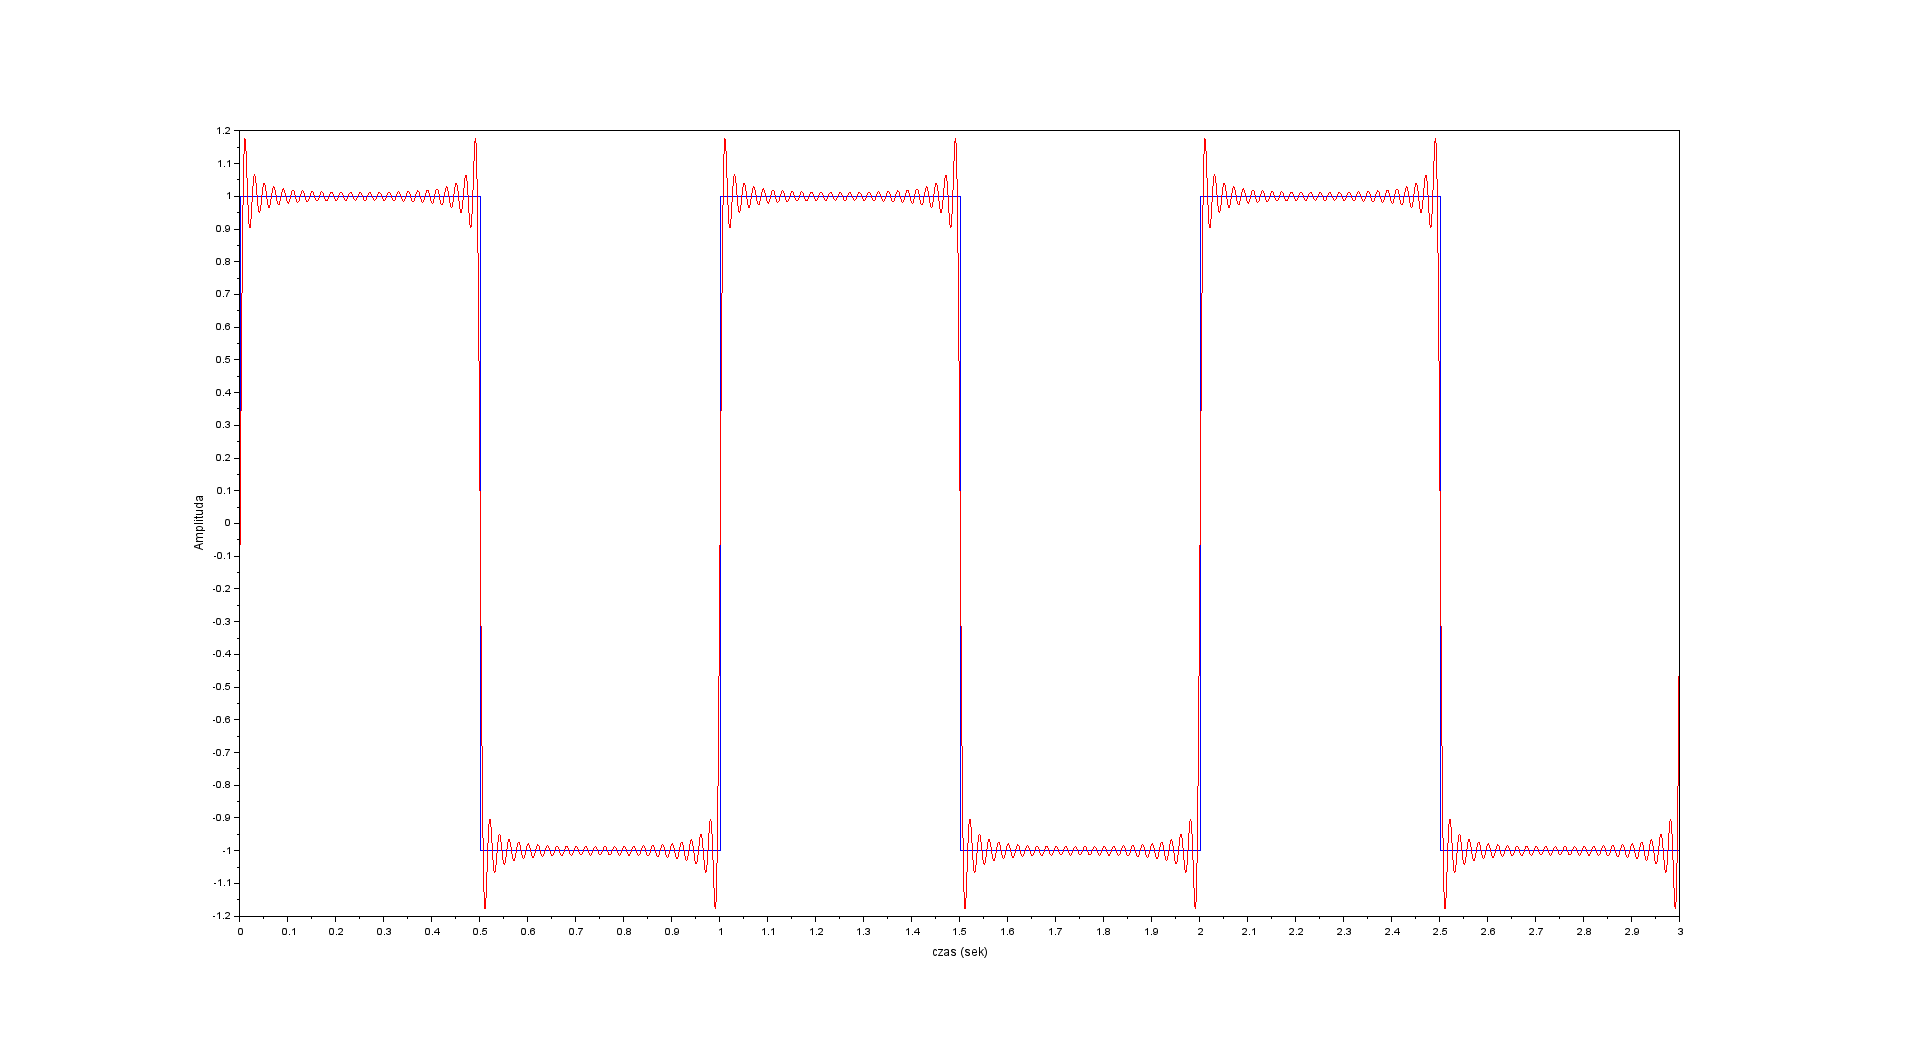
\includegraphics[width=24cm]{img/synthesis(50, 3, rectangular).png}
		\hspace*{\fill}
	\end{figure}
	
	\newpage
	Sygnał trójkątny
	\begin{minted}[linenos, fontsize=\small]{scilab}
		synthesis(5, 3, triangular)
	\end{minted}
	\begin{figure}[H]
		\centering
		\hspace*{-4.5cm}
		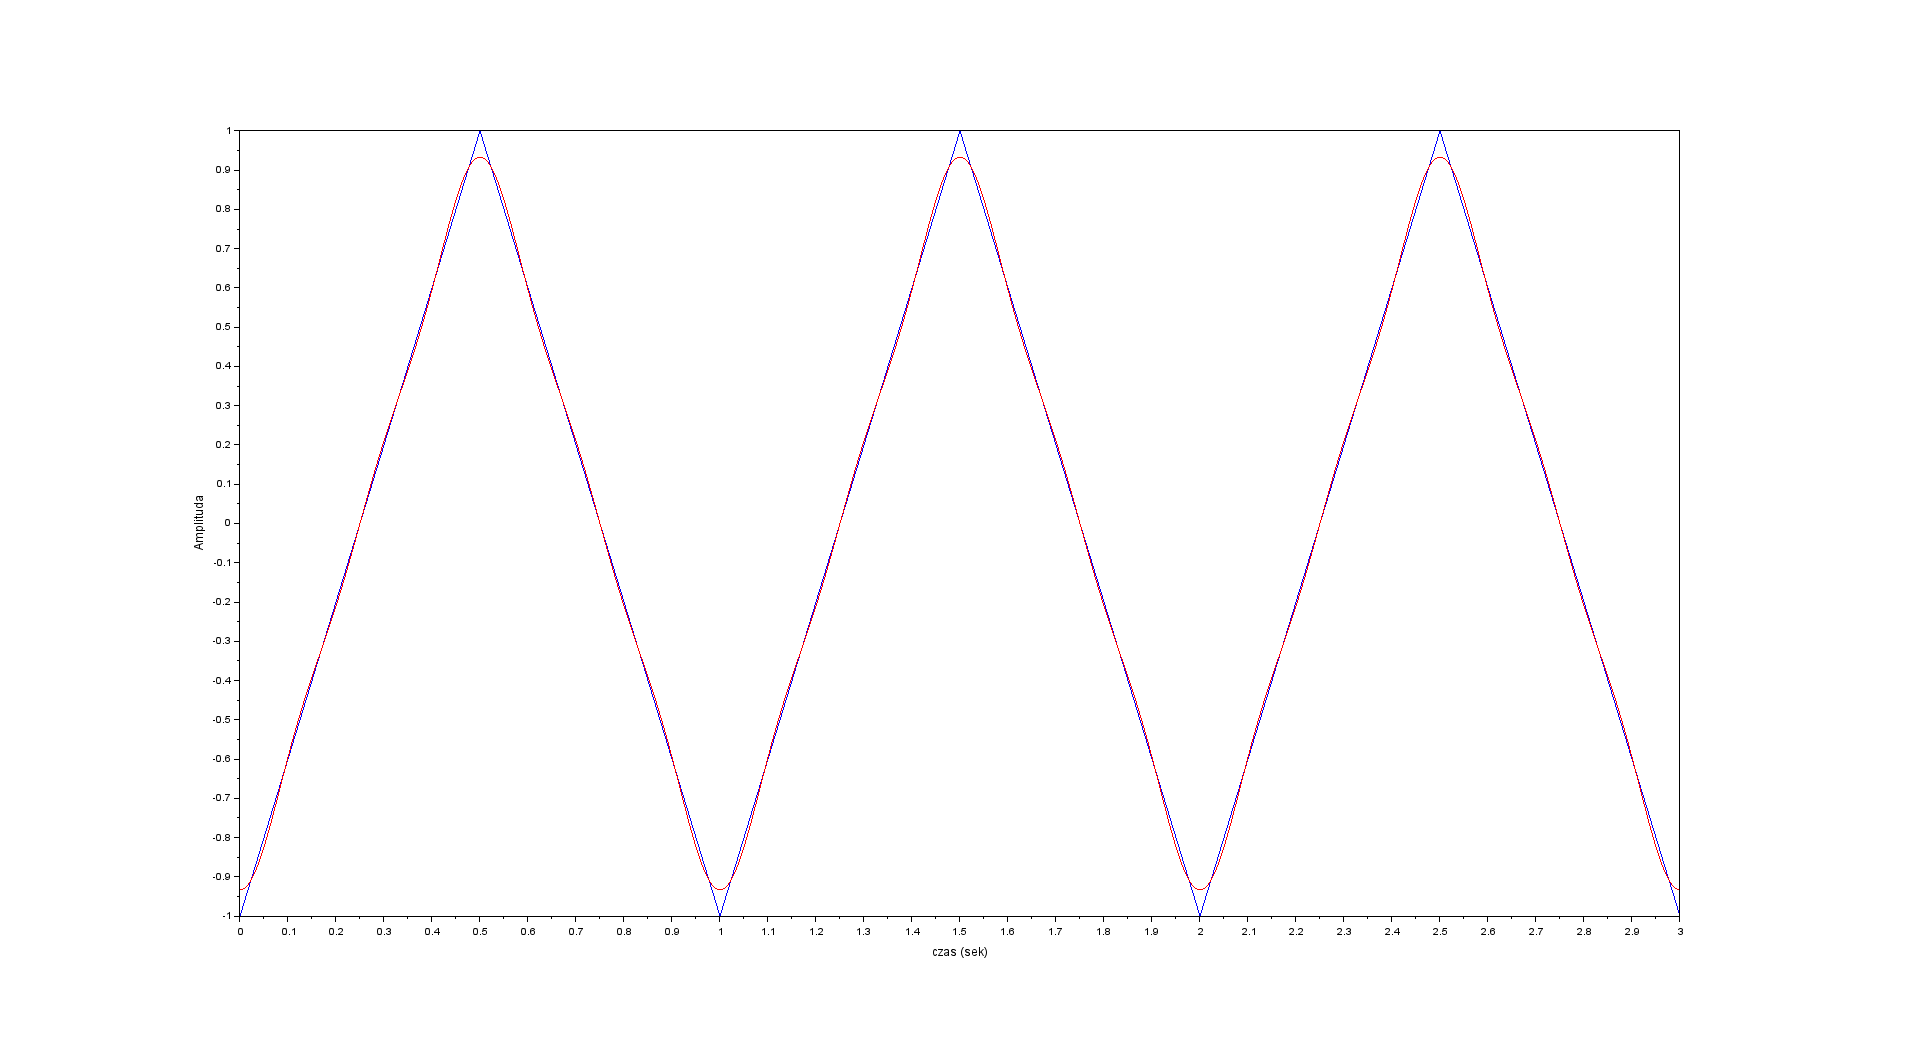
\includegraphics[width=24cm]{img/synthesis(5, 3, triangular).png}
		\hspace*{\fill}
	\end{figure}
	\newpage
	Sygnał piłokształtny
	\begin{minted}[linenos, fontsize=\small]{scilab}
		synthesis(25, 3, sawtooth)
	\end{minted}
		\begin{figure}[H]
		\centering
		\hspace*{-4.5cm}
		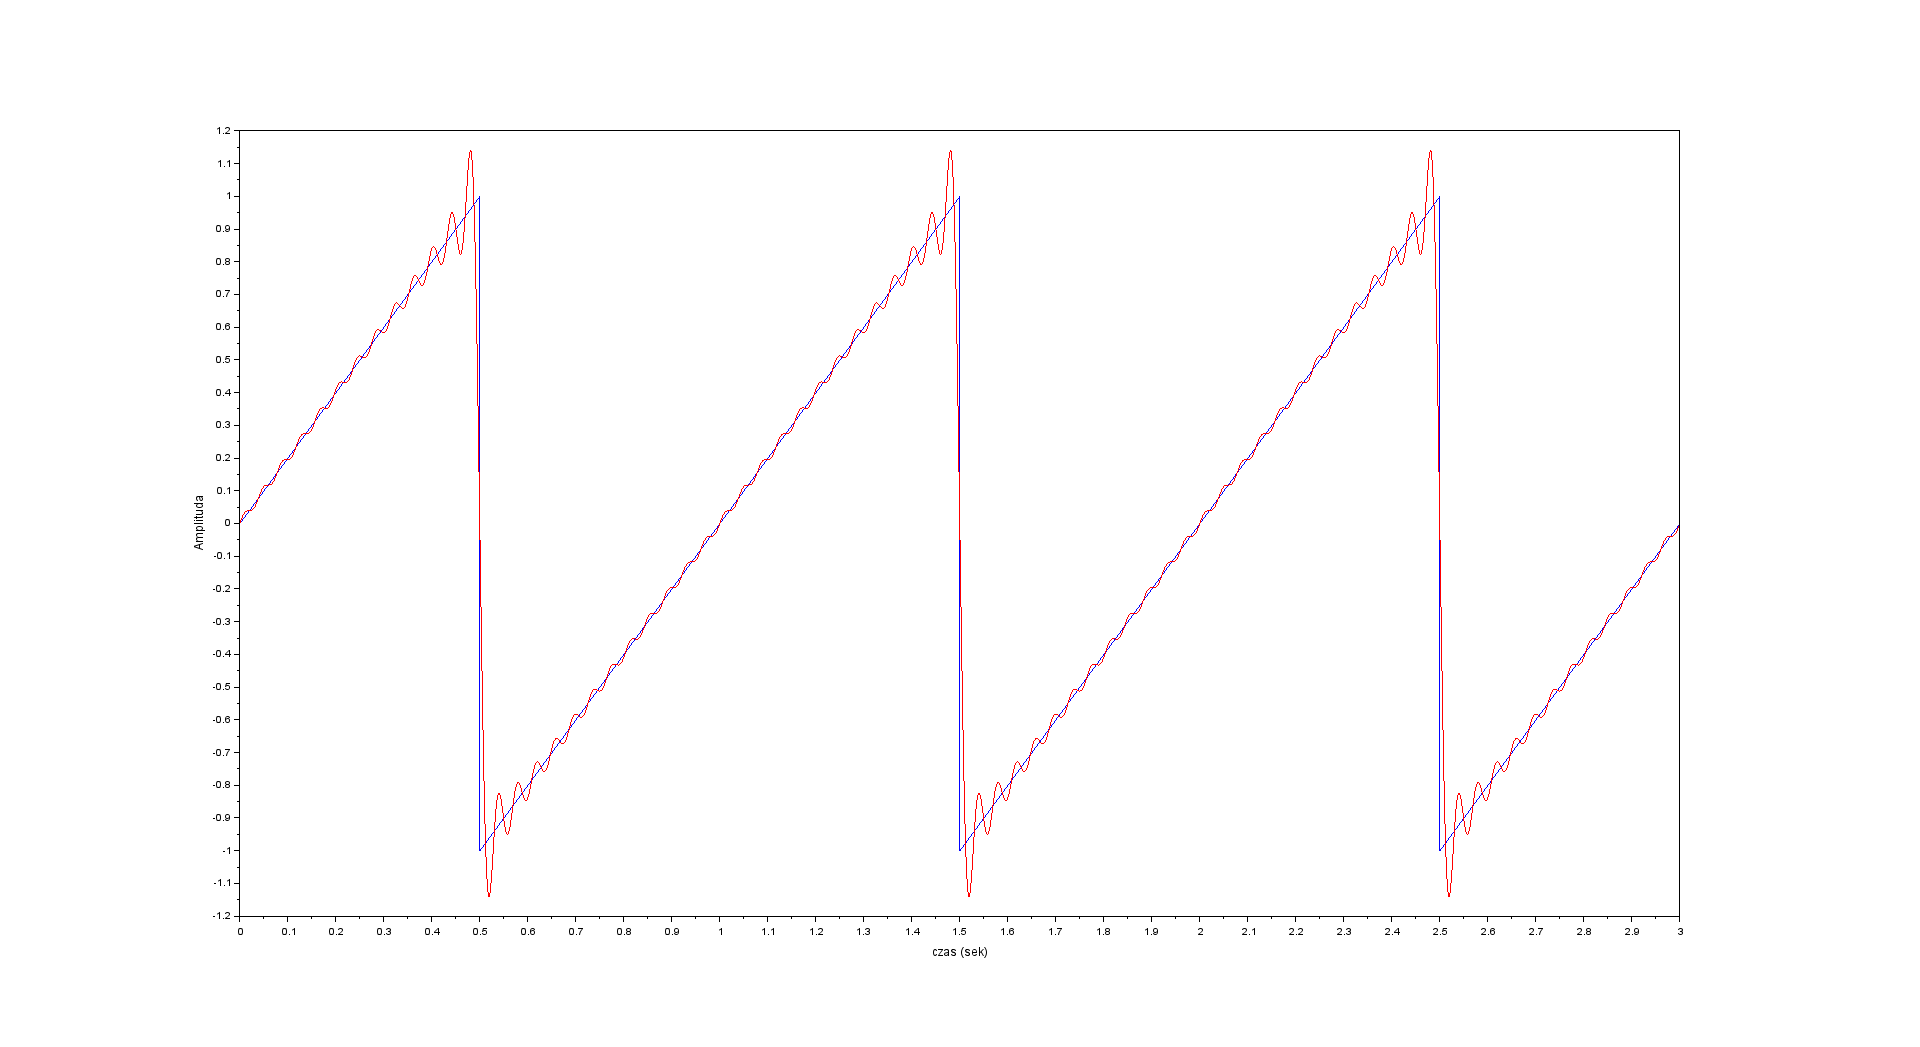
\includegraphics[width=24cm]{img/synthesis(25, 3, sawtooth).png}
		\hspace*{\fill}
	\end{figure}
	
	\section{Modulacje sygnału}
	\subsection{Modulacja amplitudy}
	Modulację amplitudy przeprowadzimy zgodnie ze wzorem
	\[
		s(t) = A[1 + k_a m(t)]\cdot x(t),
	\]
	Algorytm napisany w Scilabie wygląda następująco
	\begin{minted}[linenos, fontsize=\small]{scilab}
		function amplitude_modulation(NT, x)
		//NT - liczba okresów
		//x - wykorzystana funkcja fali
		
		ka = 0.5;               //amplituda modulacji
		T = 1;                  //okres
		N_per = 1000;           //liczba próbek na 1 okres
		N = N_per*NT;           //całkowita liczba próbek
		A = 1;                  //amplituda
		
		dt = (T * NT) / N;      //krok czasowy
		t = 0:dt:(T*NT - dt);   //oś czasu
		
		//generowanie funkcji fali z zadanymi parametrami
		xn = x(A, t, T);
		
		//generowanie sygnału modulującego
		fm = 0.1;
		m = sin(2 * %pi * fm * t);
		
		//generowanie zmodulowanego sygnału
		s = A*(1 + ka*m) .* xn .* (xn ~= 0);
		plot(t, s);
		title('Modulacja amplitudy');
		xlabel('czas (sek)');
		ylabel('Amplituda');
		endfunction
	\end{minted}
	\newpage
	Oto przykładowe wywołanie powyższej funkcji dla fali trójkątnej
	\begin{minted}[linenos, fontsize=\small]{scilab}
		amplitude_modulation(20, triangular)
	\end{minted}
	\begin{figure}[H]
		\centering
		\hspace*{-4.5cm}
		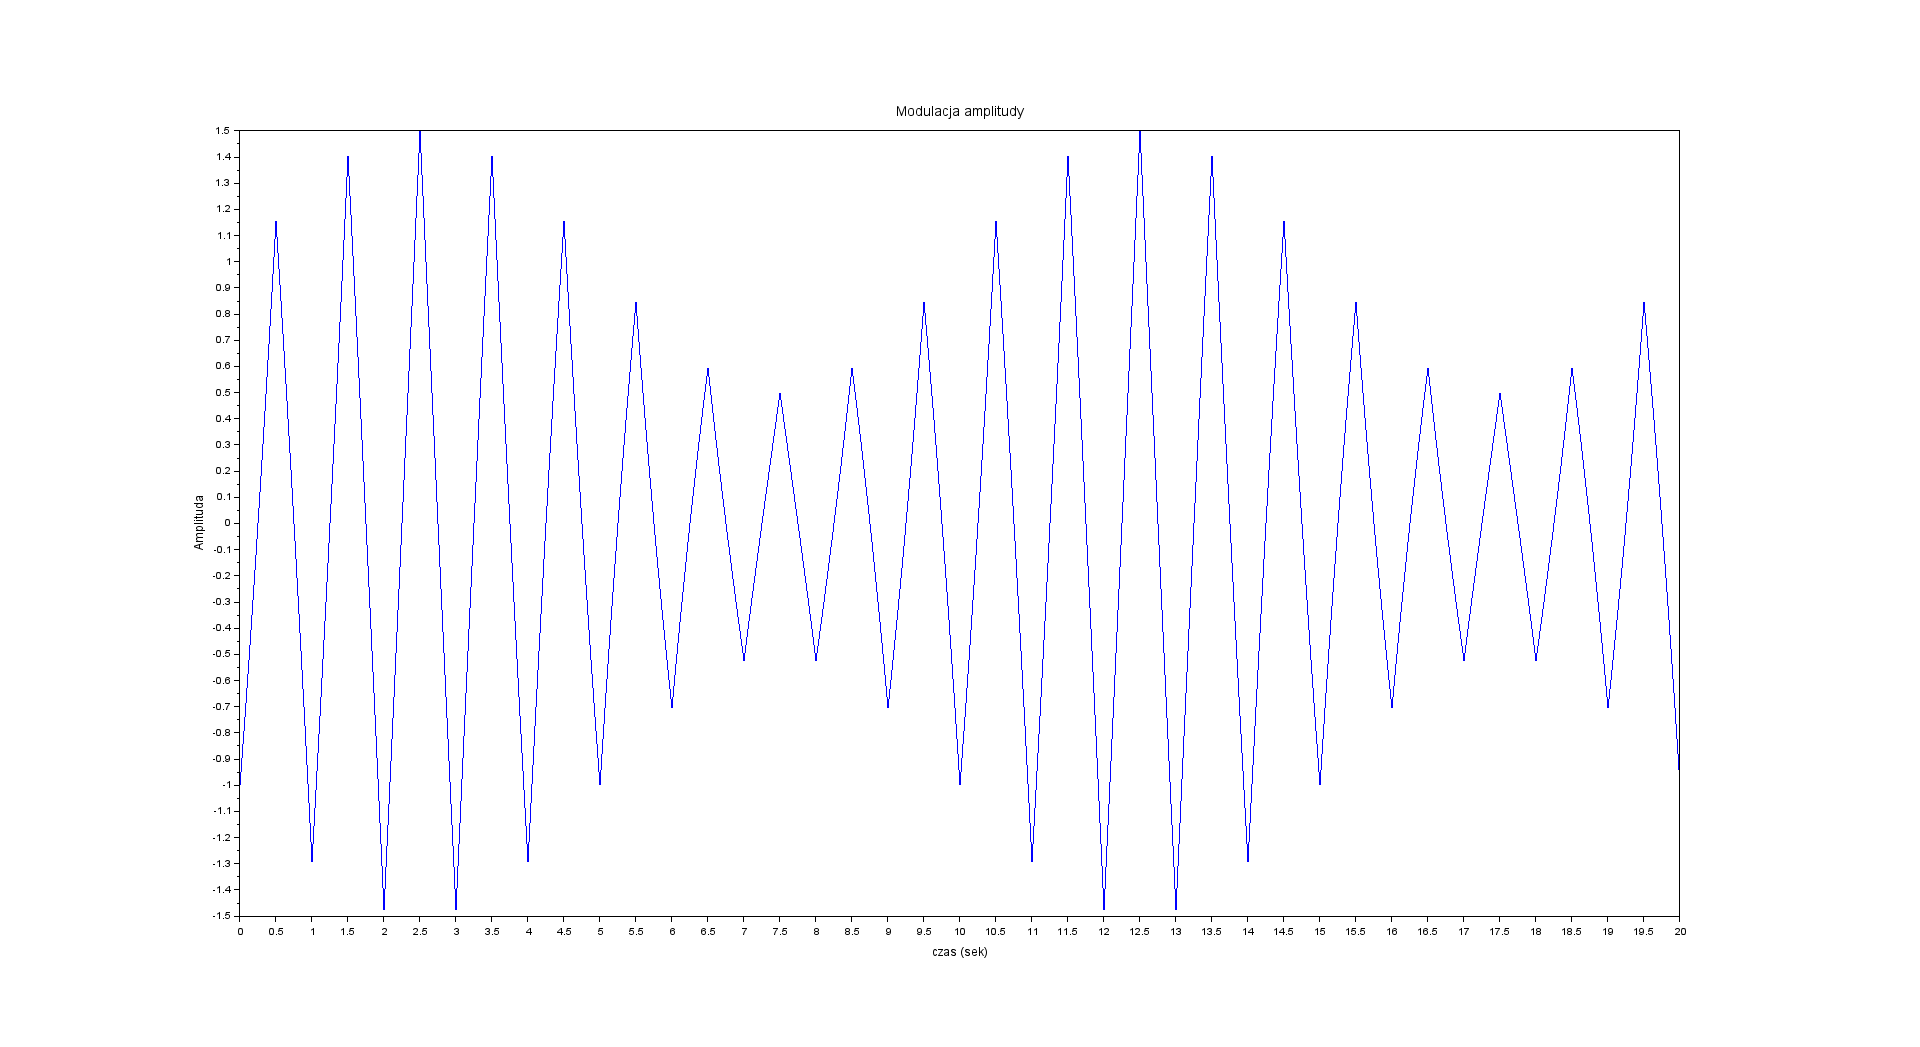
\includegraphics[width=24cm]{img/amplitude_modulation(20, triangular).png}
		\hspace*{\fill}
	\end{figure}
	
	
	\subsection{Modulacja częstotliwości}
	Modulację częstotliwości przeprowadzimy przekształcając oś czasu poprzez wyliczenie chwilowej fazy
	\[
		\phi (t) = f_c t + k_f \int_{0}^{t}m(\tau)d\tau.
	\]
	Algorytm w Scilabie wygląda następująco
	\begin{minted}[linenos, fontsize=\small]{scilab}
		function frequency_modulation(NT, x)
		//NT - liczba okresów
		//x - wykorzystana funkcja fali
		
		N_per = 1000;           //liczba próbek na 1 okres
		A = 1;                  //amplituda
		T = 1;                  //okres
		N = N_per * NT;         //całkowita liczba próbek
		fc = 1/T;               //częstotliwość nośna
		kf = 3;                 //czułość częstotliwości
		dt = (T * NT) / N;      //krok czasowy
		t = 0:dt:(T*NT - dt);   //oś czasu
		
		//generowanie sygnału modulującego
		fm = 0.5;
		m = fm*(t)^2;
		
		//obliczanie chwilowej fazy i przeskalowanie czasu
		phi = fc * t + kf * cumsum(m) * dt;
		t_fm = phi * T;
		
		//generowanie fali ze zmienną częstotliwością
		x_mod = x(A, t_fm, T);
		plot(t, x_mod);
		
		a = gca();
		a.data_bounds = [min(t), min(x_mod)-0.1; max(t), max(x_mod)+0.1];
		endfunction
	\end{minted}
	\newpage
	Oto przykładowe wywołanie powyższej funkcji dla fali prostokątnej
	\begin{minted}[linenos, fontsize=\small]{scilab}
		frequency_modulation(4, rectangular)
	\end{minted}
	\begin{figure}[H]
		\centering
		\hspace*{-4.5cm}
		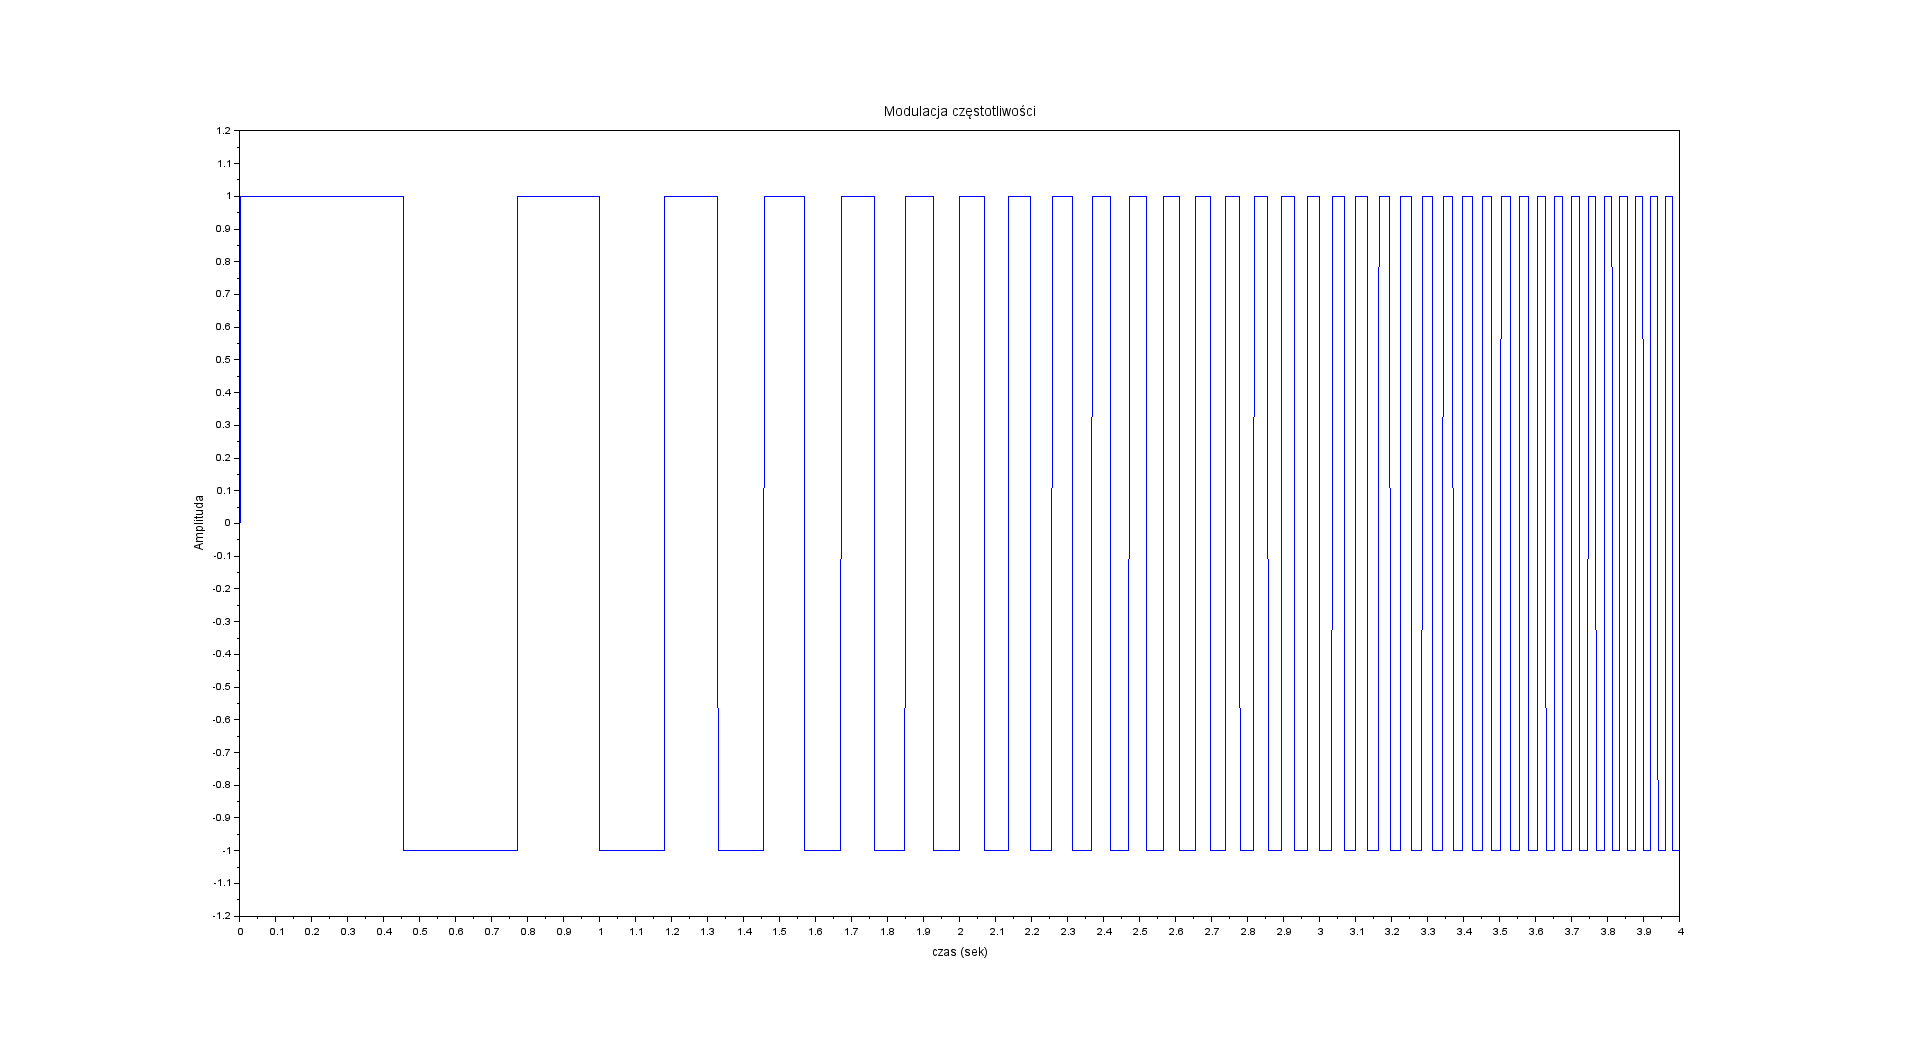
\includegraphics[width=24cm]{img/frequency_modulation(4, rectangular).png}
		\hspace*{\fill}
	\end{figure}
	
	\subsection{Modulacja fazy}
	Modulację fazy przeprowadzimy poprzez przesunięcie czasu o $\Delta t$ zależne od fazy $\phi$
	\[
		\Delta t = \phi \frac{T}{2\pi}.
	\]
	Kod w Scilabie wygląda następująco
	\begin{minted}[linenos, fontsize=\small]{scilab}
		function phase_modulation(NT, x)
		//NT - liczba okresów
		//x - wykorzystana funkcja fali
		
		N_per = 1000;           //liczba próbek na 1 okres
		N = N_per*NT;           //całkowita liczba próbek
		T = 1;                  //okres
		kp = %pi/2;             //czułość modulacji fazy
		A = 1;                  //amplituda
		dt = (T * NT) / N;      //krok czasowy
		t = 0:dt:(T*NT - dt);   //oś czasu
		
		//generowanie sygnału modulującego
		fm = 1;
		m = sin(2 * %pi * fm * t);
		//zmiana fazy
		phi = kp * m;
		x_pm = x(A, t + phi*T/(2*%pi), T); 
		
		plot(t, x_pm);
		a = gca();
		a.data_bounds = [min(t), min(x_pm)-0.1; max(t), max(x_pm)+0.1];
		endfunction
	\end{minted}
	\newpage
	Oto przykładowe wywołanie powyższej funkcji dla fali prostokątnej
	\begin{minted}[linenos, fontsize=\small]{scilab}
		phase_modulation(4, sawtooth)
	\end{minted}
	\begin{figure}[H]
		\centering
		\hspace*{-4.5cm}
		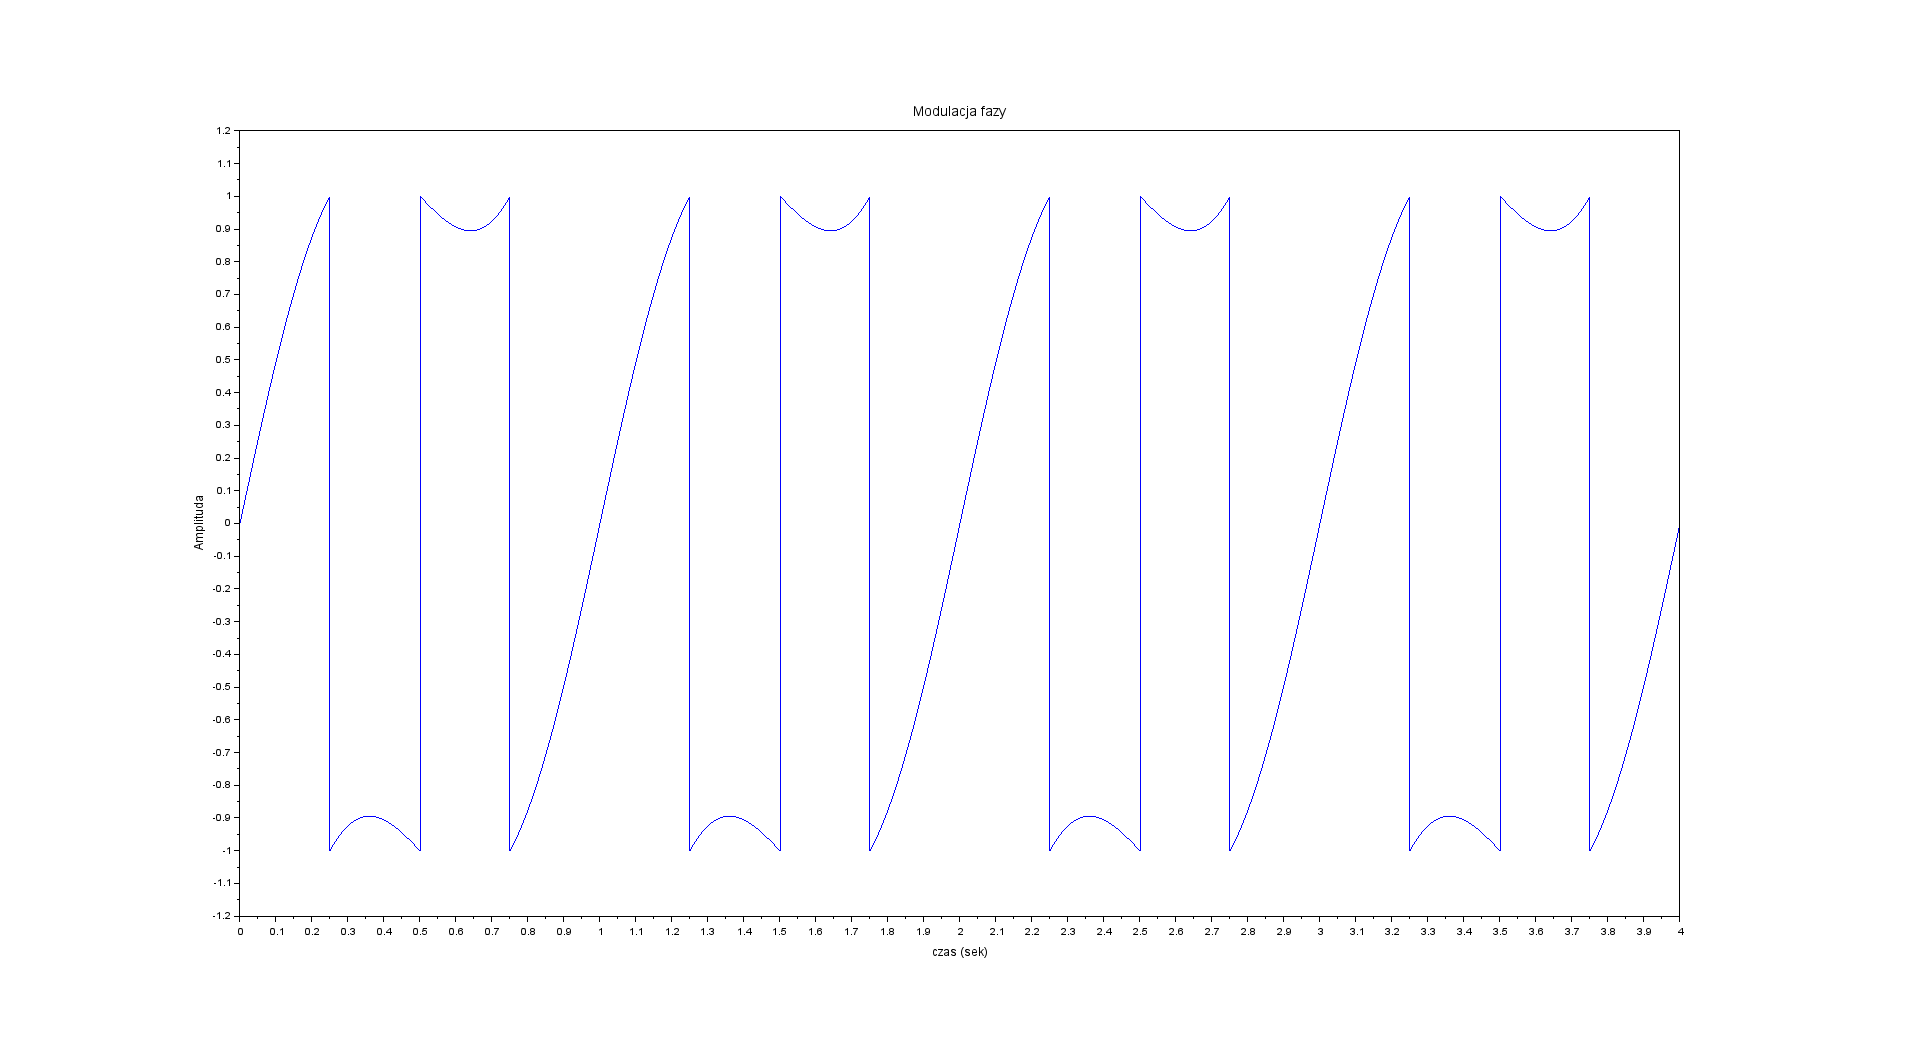
\includegraphics[width=24cm]{img/phase_modulation(4, sawtooth).png}
		\hspace*{\fill}
	\end{figure}
	
\end{document}